% Created 2020-05-25 一 12:18
% Intended LaTeX compiler: pdflatex
\documentclass[11pt]{article}
\usepackage[utf8]{inputenc}
\usepackage[T1]{fontenc}
\usepackage{graphicx}
\usepackage{grffile}
\usepackage{longtable}
\usepackage{wrapfig}
\usepackage{rotating}
\usepackage[normalem]{ulem}
\usepackage{amsmath}
\usepackage{textcomp}
\usepackage{amssymb}
\usepackage{capt-of}
\usepackage{imakeidx}
\usepackage{hyperref}
\usepackage{minted}
% TIPS
% \substack{a\\b} for multiple lines text





% pdfplots will load xolor automatically without option
\usepackage[dvipsnames]{xcolor}

\usepackage{forest}
% two-line text in node by [two \\ lines]
% \begin{forest} qtree, [..] \end{forest}
\forestset{
  qtree/.style={
    baseline,
    for tree={
      parent anchor=south,
      child anchor=north,
      align=center,
      inner sep=1pt,
    }}}
%\usepackage{flexisym}
% load order of mathtools and mathabx, otherwise conflict overbrace

\usepackage{mathtools}
%\usepackage{fourier}
\usepackage{pgfplots}
\usepackage{amsthm}
\usepackage{amsmath}
%\usepackage{unicode-math}
%
\usepackage{commath}
%\usepackage{,  , }
\usepackage{amsfonts}
\usepackage{amssymb}
% importing symbols https://tex.stackexchange.com/questions/14386/importing-a-single-symbol-from-a-different-font
%mathabx change every symbol
% use instead stmaryrd
%\usepackage{mathabx}
\usepackage{stmaryrd}
\usepackage{empheq}
\usepackage{tikz}
\usepackage{tikz-cd}
%\usepackage[notextcomp]{stix}
\usetikzlibrary{arrows.meta}
\usepackage[most]{tcolorbox}
%\utilde
%\usepackage{../../latexpackage/undertilde/undertilde}
% left and right superscript and subscript
\usepackage{actuarialsymbol}
\usepackage{threeparttable}
\usepackage{scalerel,stackengine}
\usepackage{stackrel}
% \stackrel[a]{b}{c}
\usepackage{dsfont}
% text font
\usepackage{newpxtext}
%\usepackage{newpxmath}

%\newcounter{dummy} \numberwithin{dummy}{section}
\newtheorem{dummy}{dummy}[section]
\theoremstyle{definition}
\newtheorem{definition}[dummy]{Definition}
\newtheorem{corollary}[dummy]{Corollary}
\newtheorem{lemma}[dummy]{Lemma}
\newtheorem{proposition}[dummy]{Proposition}
\newtheorem{theorem}[dummy]{Theorem}
\theoremstyle{definition}
\newtheorem{example}[dummy]{Example}
\theoremstyle{remark}
\newtheorem*{remark}{Remark}


\newcommand\what[1]{\ThisStyle{%
    \setbox0=\hbox{$\SavedStyle#1$}%
    \stackengine{-1.0\ht0+.5pt}{$\SavedStyle#1$}{%
      \stretchto{\scaleto{\SavedStyle\mkern.15mu\char'136}{2.6\wd0}}{1.4\ht0}%
    }{O}{c}{F}{T}{S}%
  }
}

\newcommand\wtilde[1]{\ThisStyle{%
    \setbox0=\hbox{$\SavedStyle#1$}%
    \stackengine{-.1\LMpt}{$\SavedStyle#1$}{%
      \stretchto{\scaleto{\SavedStyle\mkern.2mu\AC}{.5150\wd0}}{.6\ht0}%
    }{O}{c}{F}{T}{S}%
  }
}

\newcommand\wbar[1]{\ThisStyle{%
    \setbox0=\hbox{$\SavedStyle#1$}%
    \stackengine{.5pt+\LMpt}{$\SavedStyle#1$}{%
      \rule{\wd0}{\dimexpr.3\LMpt+.3pt}%
    }{O}{c}{F}{T}{S}%
  }
}

\newcommand{\bl}[1] {\boldsymbol{#1}}
\newcommand{\Wt}[1] {\stackrel{\sim}{\smash{#1}\rule{0pt}{1.1ex}}}
\newcommand{\wt}[1] {\widetilde{#1}}
\newcommand{\tf}[1] {\textbf{#1}}


%For boxed texts in align, use Aboxed{}
%otherwise use boxed{}

\DeclareMathSymbol{\widehatsym}{\mathord}{largesymbols}{"62}
\newcommand\lowerwidehatsym{%
  \text{\smash{\raisebox{-1.3ex}{%
    $\widehatsym$}}}}
\newcommand\fixwidehat[1]{%
  \mathchoice
    {\accentset{\displaystyle\lowerwidehatsym}{#1}}
    {\accentset{\textstyle\lowerwidehatsym}{#1}}
    {\accentset{\scriptstyle\lowerwidehatsym}{#1}}
    {\accentset{\scriptscriptstyle\lowerwidehatsym}{#1}}
}

\usepackage{graphicx}
    
% text on arrow for xRightarrow
\makeatletter
%\newcommand{\xRightarrow}[2][]{\ext@arrow 0359\Rightarrowfill@{#1}{#2}}
\makeatother


\newcommand{\dom}[1]{%
\mathrm{dom}{(#1)}
}

% Roman numerals
\makeatletter
\newcommand*{\rom}[1]{\expandafter\@slowromancap\romannumeral #1@}
\makeatother

\def \fR {\mathfrak{R}}
\def \bx {\boldsymbol{x}}
\def \bz {\boldsymbol{z}}
\def \ba {\boldsymbol{a}}
\def \bh {\boldsymbol{h}}
\def \bo {\boldsymbol{o}}
\def \bU {\boldsymbol{U}}
\def \bc {\boldsymbol{c}}
\def \bV {\boldsymbol{V}}
\def \bI {\boldsymbol{I}}
\def \bK {\boldsymbol{K}}
\def \bt {\boldsymbol{t}}
\def \bb {\boldsymbol{b}}
\def \bA {\boldsymbol{A}}
\def \bX {\boldsymbol{X}}
\def \bu {\boldsymbol{u}}
\def \bS {\boldsymbol{S}}
\def \bZ {\boldsymbol{Z}}
\def \bz {\boldsymbol{z}}
\def \by {\boldsymbol{y}}
\def \bw {\boldsymbol{w}}
\def \bT {\boldsymbol{T}}
\def \bF {\boldsymbol{F}}
\def \bS {\boldsymbol{S}}
\def \bm {\boldsymbol{m}}
\def \bW {\boldsymbol{W}}
\def \bR {\boldsymbol{R}}
\def \bQ {\boldsymbol{Q}}
\def \bS {\boldsymbol{S}}
\def \bP {\boldsymbol{P}}
\def \bT {\boldsymbol{T}}
\def \bY {\boldsymbol{Y}}
\def \bH {\boldsymbol{H}}
\def \bB {\boldsymbol{B}}
\def \blambda {\boldsymbol{\lambda}}
\def \bPhi {\boldsymbol{\Phi}}
\def \btheta {\boldsymbol{\theta}}
\def \bTheta {\boldsymbol{\Theta}}
\def \bmu {\boldsymbol{\mu}}
\def \bphi {\boldsymbol{\phi}}
\def \bSigma {\boldsymbol{\Sigma}}
\def \lb {\left\{}
\def \rb {\right\}}
\def \la {\langle}
\def \ra {\rangle}
\def \caln {\mathcal{N}}
\def \dissum {\displaystyle\Sigma}
\def \dispro {\displaystyle\prod}
\def \E {\mathbb{E}}
\def \Q {\mathbb{Q}}
\def \N {\mathbb{N}}
\def \V {\mathbb{V}}
\def \R {\mathbb{R}}
\def \P {\mathbb{P}}
\def \A {\mathbb{A}}
\def \Z {\mathbb{Z}}
\def \I {\mathbb{I}}
\def \C {\mathbb{C}}
\def \cala {\mathcal{A}}
\def \calb {\mathcal{B}}
\def \calq {\mathcal{Q}}
\def \calp {\mathcal{P}}
\def \cals {\mathcal{S}}
\def \calg {\mathcal{G}}
\def \caln {\mathcal{N}}
\def \calr {\mathcal{R}}
\def \calm {\mathcal{M}}
\def \calc {\mathcal{C}}
\def \calf {\mathcal{F}}
\def \calk {\mathcal{K}}
\def \call {\mathcal{L}}
\def \calu {\mathcal{U}}
\def \bcup {\bigcup}


\def \uin {\underline{\in}}
\def \oin {\overline{\in}}
\def \uR {\underline{R}}
\def \oR {\overline{R}}
\def \uP {\underline{P}}
\def \oP {\overline{P}}

\def \Ra {\Rightarrow}

\def \e {\enspace}

\def \sgn {\operatorname{sgn}}
\def \gen {\operatorname{gen}}
\def \ker {\operatorname{ker}}
\def \im {\operatorname{im}}

\def \tril {\triangleleft}

% \varprod
\DeclareSymbolFont{largesymbolsA}{U}{txexa}{m}{n}
\DeclareMathSymbol{\varprod}{\mathop}{largesymbolsA}{16}

% \bigtimes
\DeclareFontFamily{U}{mathx}{\hyphenchar\font45}
\DeclareFontShape{U}{mathx}{m}{n}{
      <5> <6> <7> <8> <9> <10>
      <10.95> <12> <14.4> <17.28> <20.74> <24.88>
      mathx10
      }{}
\DeclareSymbolFont{mathx}{U}{mathx}{m}{n}
\DeclareMathSymbol{\bigtimes}{1}{mathx}{"91}
% \odiv
\DeclareFontFamily{U}{matha}{\hyphenchar\font45}
\DeclareFontShape{U}{matha}{m}{n}{
      <5> <6> <7> <8> <9> <10> gen * matha
      <10.95> matha10 <12> <14.4> <17.28> <20.74> <24.88> matha12
      }{}
\DeclareSymbolFont{matha}{U}{matha}{m}{n}
\DeclareMathSymbol{\odiv}         {2}{matha}{"63}


\newcommand\subsetsim{\mathrel{%
  \ooalign{\raise0.2ex\hbox{\scalebox{0.9}{$\subset$}}\cr\hidewidth\raise-0.85ex\hbox{\scalebox{0.9}{$\sim$}}\hidewidth\cr}}}
\newcommand\simsubset{\mathrel{%
  \ooalign{\raise-0.2ex\hbox{\scalebox{0.9}{$\subset$}}\cr\hidewidth\raise0.75ex\hbox{\scalebox{0.9}{$\sim$}}\hidewidth\cr}}}

\newcommand\simsubsetsim{\mathrel{%
  \ooalign{\raise0ex\hbox{\scalebox{0.8}{$\subset$}}\cr\hidewidth\raise1ex\hbox{\scalebox{0.75}{$\sim$}}\hidewidth\cr\raise-0.95ex\hbox{\scalebox{0.8}{$\sim$}}\cr\hidewidth}}}
\newcommand{\stcomp}[1]{{#1}^{\mathsf{c}}}


\author{David Marker}
\date{\today}
\title{Model Theory: An Introduction}
\hypersetup{
 pdfauthor={David Marker},
 pdftitle={Model Theory: An Introduction},
 pdfkeywords={},
 pdfsubject={},
 pdfcreator={Emacs 26.3 (Org mode 9.3.6)}, 
 pdflang={English}}
\begin{document}

\maketitle \clearpage
\tableofcontents \clearpage\section{Structures and Theories}
\label{sec:org3967d19}
\subsection{Languages and Structures}
\label{sec:orgadfa42b}
\begin{definition}[]
A language \(\call\) is given by specifying the following data
\begin{enumerate}
\item A set of function symbols \(\calf\) and positive integers \(n_f\) for each
\(f\in\calf\)
\item a set of relation symbols \(\calr\) and positive integers \(n_R\) for each
\(R\in\calr\)
\item a set of constant symbols \(\calc\)
\end{enumerate}
\end{definition}

\begin{definition}[]
An \(\call\)-structure \(\calm\) is given by the following data
\begin{enumerate}
\item a nonempty set \(M\) called the \textbf{universe}, \textbf{domain} or \textbf{underlying set}
of \(\calm\)
\item a function \(f^\calm:M^{n_f}\to M\) for each \(f\in\calf\)
\item a set \(R^\calm\subseteq M^{n_R}\) for each \(R\in\calr\)
\item an element \(c^\calm\in M\) for each \(c\in\calc\)
\end{enumerate}
\end{definition}

We refer to \(f^\calm,R^\calm,c^\calm\) as the \textbf{interpretations} of the
symbols \(f,R\) and \(c\). We often write the structure as
\(\calm=(M,f^\calm,R^\calm,c^\calm:f\in\calf,R\in\calr,c\in\calc)\) 

\begin{definition}[]
Suppose that \(\calm\) and \(\caln\) are \(\call\)-structures with universes \(M\)
and \(N\) respectively. An \textbf{\(\call\)-embedding} \(\eta:\calm\to\caln\) is a
one-to-one map \(\eta:M\to N\) that
\begin{enumerate}
\item \(\eta(f^\calm(a_1,\dots,a_{n_f}))=f^\caln(\eta(a_1),\dots,\eta(a_{n_f}))\)
for all \(f\in\calf\) and \(a_1,\dots,a_{n_f}\in M\)
\item \((a_1,\dots,a_{m_R})\in R^\calm\) if and only if
\((\eta(a_1),\dots,\eta(a_{m_R}))\in R^\caln\) for all \(R\in\calr\) and
\(a_1,\dots,a_{m_R}\in M\)
\item \(\eta(c^\calm)=c^\caln\) for \(c\in\calc\)
\end{enumerate}
\end{definition}

A bijective \(\call\)-embedding is called an \textbf{\(\call\)-isomorphism}. If
\(M\subseteq N\) and the inclusion map is an \(\call\)-embedding, we say either
\(\calm\) is a \textbf{substrcture} of \(\caln\) or that \(\caln\) is an \textbf{extension}
of \(\calm\)

The \textbf{cardinality} of \(\calm\) is \(\abs{M}\), the cardinality of the universe of \(\calm\)

\begin{definition}[]
The set of \textbf{\(\call\)-terms} is the smallest set \(\calt\) s.t.
\begin{enumerate}
\item \(c\in\calt\) for each constant symbol \(c\in\calc\)
\item each variable symbol \(v_i\in\calt\) for \(i=1,2,\dots\)
\item if \(t_1,\dots,t_{n_f}\in\calt\) and \(f\in\calf\) then
\(f(t_1,\dots,n_{n_f})\in\calt\)
\end{enumerate}
\end{definition}


Suppose that \(\calm\) is an \(\call\)-structure and that \(t\) is a term built
using variables from \(\bar{v}=(v_{i_1},\dots,v_{i_m})\). We want to interpret
\(t\) as a function \(t^\calm:M^m\to M\). For \(s\) a subterm of \(t\) and
\(\bar{a}=(a_{i_1},\dots,a_{i_m})\in M\), we inductively define
\(s^\calm(\bar{a})\) as follows.
\begin{enumerate}
\item If \(s\) is a constant symbol \(c\), then \(s^\calm(\bar{a})=c^\calm\)
\item If \(s\) is the variable \(v_{i_j}\), then \(s^\calm(\bar{a})=a_{i_j}\)
\item If \(s\) is the term \(f(t_1,\dots,t_{n_f})\), where \(f\) is a function symbol
of \(\call\) and \(t_1,\dots,t_{n_f}\) are terms, then 
\(s^\calm(\bar{a})=f^\calm(t^\calm_1(\bar{a}),\dots,t_{n_f}^\calm(\bar{a}))\)
\end{enumerate}


The function \(t^\calm\) is defined by \(\bar{a}\mapsto t^\calm(\bar{a})\)


\begin{definition}[]
\(\phi\) is an \textbf{atomic} \textbf{\(\call\)-formula} if \(\phi\) is either
\begin{enumerate}
\item \(t_1=t_2\) where \(t_1\) and \(t_2\) are terms
\item \(R(t_1,\dots,t_{n_R})\)
\end{enumerate}


The set of \textbf{\(\call\)-formulas} is the smallest set \(\calw\) containing the
atomic formulas s.t.
\begin{enumerate}
\item if \(\phi\in\calw\), then \(\neg\phi\in\calw\)
\item if \(\phi,\psi\in\calw\), then \((\phi\wedge\psi),(\phi\vee\psi)\in\calw\)
\item if \(\phi\in\calw\), then \(\exists v_i\phi,\forall v_i\phi\in\calw\)
\end{enumerate}
\end{definition}

We say a variable \(v\) \textbf{occurs freely} in a formula \(\phi\) if it is not
inside a \(\exists v\) or \(\forall v\) quantifier; otherwise we say that it's
\textbf{bound}. We call a formula a \textbf{sentence} if it has no free variables. We
often write \(\phi(v_1,\dots,v_n)\) to make explicit the free variables in \(\phi\)

\begin{definition}[]
Let \(\phi\) be a formula with free variables from
\(\bar{v}=(v_{i_1,\dots,v_{i_m}})\) and let \(\bar{a}=(a_{i_1},\dots,a_{i_m})\in
   M^m\). We inductively define \(\calm\models\phi\bar{a}\) as follows
\begin{enumerate}
\item If \(\phi\) is \(t_1=t_2\), then \(\calm\models\phi(\bar{a})\) if
\(t_1^\calm(\bar{a})=t_2^\calm(\bar{a})\)
\item If \(\phi\) is \(R(t_1,\dots,t_{m_R})\) then \(\calm\models\phi(\bar{a})\) if
\((t_1^\calm(\bar{a}),\dots,t_{m_R}^\calm(\bar{a}))\in R^\calm\)
\item If \(\phi\) is \(\neg\psi\) then \(\calm\models\phi(\bar{a})\) if
\(\calm\not\models\psi(\bar{a})\)
\item If \(\phi\) is \((\psi\wedge\theta)\) then \(\calm\models\phi(\bar{a})\) if
\(\calm\models\psi(\bar{a})\) and
\(\calm\models\theta(\bar{a})\)
\item If \(\phi\) is \((\psi\vee\theta)\) then \(\calm\models\phi(\bar{a})\) if
\(\calm\models\psi(\bar{a})\) or
\(\calm\models\theta(\bar{a})\)
\item If \(\phi\) is \(\exists v_j\psi(\bar{v},v_j)\) then \(\calm\models\phi(\bar{a})\)
if there is \(b\in M\) s.t. \(\calm\models\psi(\bar{a},b)\)
\item If \(\phi\) is \(\forall v_j\psi(\bar{v},v_j)\) then \(\calm\models\phi(\bar{a})\)
if \(\calm\models\psi(\bar{a},b)\) for all \(b\in M\)
\end{enumerate}
\end{definition}


If \(\calm\models\phi(\bar{a})\) we say that \(\calm\) \textbf{satisfies}
\(\phi(\bar{a})\) or \(\phi(\bar{a})\) is \textbf{true} in \(\calm\)

\begin{proposition}[]
Suppose that \(\calm\) is a substrcture of \(\caln\), \(\bar{a}\in M\) and
\(\phi(\bar{v})\) is a quantifier-free formula. Then
\(\calm\models\phi(\bar{a})\) if and only if \(\caln\models\psi(\bar{a})\)
\end{proposition}

\begin{proof}
\textbf{Claim} If \(t(\bar{v})\) is a term and \(\bar{b}\in M\) then
\(t^\calm(\bar{b})=t^\caln(\bar{b})\). 
\end{proof}

\begin{definition}[]
We say that two \(\call\)-strctures \(\calm\) and \(\caln\) are \textbf{elementarily}
\textbf{equivalent} and write \(\calm\equiv\caln\) if
\begin{equation*}
 \calm\models\phi\text{ if and only if } \caln\models\phi
\end{equation*}
for all \(\call\)-sentences \(\phi\)
\end{definition}

\index{full theory}
We let \(\Th(\calm)\), the \textbf{full theory} of \(\calm\) be the set of
\(\call\)-sentences \(\phi\) s.t. \(\calm\models\phi\)

\begin{theorem}[]
\label{thm1.1.10}
Suppose that \(j:\calm\to\caln\) is an isomorphism. Then \(\calm\equiv\caln\)
\end{theorem}

\begin{proof}
Show by induction on formulas that \(\calm\models\phi(a_1,\dots,a_n)\) if and
only if \(\caln\models\phi(j(a_1),\dots,j(a_n))\) for all formulas \(\phi\)
\end{proof}
\subsection{Theories}
\label{sec:org517f627}
\index{model}
\index{satisfiable}
Let \(\call\) be a language. An \textbf{\(\call\)-theory} \(T\) is a set of
\(\call\)-sentences. We say that \(\calm\) is a \textbf{model} of \(T\) and write
\(\calm\models T\) if \(\calm\models\phi\) for all sentences \(\phi\in T\). A
theory is \textbf{satisfiable} if it has a model.

\index{elementary class}
A class of \(\call\)-structures \(\calk\) is an \textbf{elementary class} if there
is an \(\call\)-theory \(T\) s.t. \(\calk=\{\calm:\calm\models T\}\)
\begin{examplle}[Groups]
Let \(\call=\{\cdot,e\}\) where \(\cdot\) is a binary function symbol and \(e\) is a 
constant symbol. The class of groups is axiomatized by
\begin{align*}
&\forall x\;e\cdot x=x\cdot e=x\\
&\forall x\forall y\forall z\;x\cdot(y\cdot z)=(x\cdot y)\cdot z\\
&\forall x\exists y\;x\cdot y=y\cdot x= e
\end{align*}
\end{examplle}

\begin{examplle}[Left \(R\)-modules]
Let \(R\) be a ring with multiplicative identity 1. Let
\(\call=\{+,0\}\cup\{r:r\in R\}\) where \(+\) is a binary function symbol, 0 is a
constant, and \(r\) is a unary function symbol for \(r\in R\). In an
\(R\)-module, we will interpret \(r\) as scalar multiplication by \(R\). The
axioms for \(R\)-modules are
\begin{align*}
&\forall x\e r(x+y)=r(x)+r(y)\text{ for each }r\in R\\
&\forall x\e (r+s)(x)=r(x)+s(x)\text{ for each }r,s\in R\\
&\forall x\e r(s(x))=rs(x)\text{ for } r,s\in R\\
&\forall x\e 1(x)=x
\end{align*}
\end{examplle}
\begin{examplle}[Rings and Fields]
Let \(\call_r\) be the language of rings \(\{+,-,\cdot,0,1\}\), where \(+,-\) and \(\cdot\)
are binary function symbols and \(0\) and \(1\) are constants. The axioms for rings are given 
by
\begin{align*}
&\forall x\forall y\forall z\;(x-y=z\leftrightarrow x=y+z)\\
&\forall x\;x\cdot 0=0\\
&\forall x\forall y\forall z\;x\cdot(y\cdot z)=(x\cdot y)\cdot z\\
&\forall x\;x\cdot 1=1\cdot x=x\\
&\forall x\forall y\forall z\;x\cdot(y+z)=(x\cdot y)+(x\cdot z)\\
&\forall x\forall y\forall z\;(x+y)\cdot z=(x\cdot z)+(y\cdot z)
\end{align*}
We axiomatize the class of fields by adding
\begin{align*}
&\forall x\forall y\;x\cdot y=y\cdot x\\
&\forall x\;(x\neq 0\to\exists y\;x\cdot y=1)
\end{align*}
We axiomatize the class of algebraically closed fields by adding to the field axioms the sentences
\begin{equation*}
\forall a_0\dots\forall a_{n-1}\exists x\;x^n+\displaystyle\sum_{i=1}^{n-1}
a_ix^i=0
\end{equation*}
for \(n=1,2,\dots\). Let \(\ACF\) be the axioms for algebraically closed fields.

Let \(\psi_p\) be the \(\call_r\)-sentence \(\forall x\;
   \underbrace{x+\dots+x}_{p\text{-times}}=0\), which asserts that a field has characteristic
\(p\). For \(p>0\) a prime, let \(\ACF_p=\ACF\cup\{\psi_p\}\) and
\(\ACF_0=\ACF\cup\{\neg\psi_p:p>0\}\) be the theories of algebraically
closed fields of characteristic \(p\) and zero respectively
\end{examplle}

\begin{definition}[]
Let \(T\) be an \(\call\)-theory and \(\phi\) an \(\call\)-sentence. We say that
\(\phi\) is a \textbf{logical consequence} of \(T\) and write \(T\models\phi\) if
\(\calm\models\phi\) whenever \(\calm\models T\)
\end{definition}

\begin{proposition}[]
\begin{enumerate}
\item Let \(\call=\{+,<,0\}\) and let \(T\) be the theory of ordered abelian groups.
Then \(\forall x(x\neq 0\to x+x\neq 0)\) is a logical consequence of \(T\)
\item Let \(T\) be the theory of groups where every element has order 2. Then\par
\(T\not\models\exists x_1\exists x_2\exists x_3(x_1\neq x_2\wedge
      x_2\neq x_3\wedge x_1\neq x_3)\)
\end{enumerate}
\end{proposition}

\begin{proof}
\begin{enumerate}
\item \(\Z/2\Z\models T\wedge\neg\exists x_1\exists x_2\exists x_3(x_1\neq x_2\wedge
      x_2\neq x_3\wedge x_1\neq x_3)\)
\end{enumerate}
\end{proof}
\subsection{Definable Sets and Interpretability}
\label{sec:orgd1a7716}
\index{definable}
\begin{definition}[]
Let \(\calm=(M,\dots)\) be an \(\call\)-structure. We say that \(X\subseteq M^n\)
is \textbf{definable} if and only if there is an \(\call\)-formula 
\(\phi(v_1,\dots,v_n,w_1,\dots,w_m)\) and \(\bar{b}\in M^b\) s.t. 
\(X=\{\bar{a}\in M^n:\calm\models\phi(\bar{a},\bar{b})\}\). We say that
\(\phi(\bar{v},\bar{b})\) \textbf{defines} \(X\). We say that \(X\) is
\textbf{\(A\)-definable} or \textbf{definable over}  \(A\) if there is a formula 
\(\psi(\bar{v},w_1,\dots,w_l)\) and \(\bar{b}\in A^l\) s.t.
\(\psi(\bar{v},\bar{b})\) defines \(X\)
\end{definition}

A number of examples using \(\call_r\), the language of rings
\begin{itemize}
\item Let \(\calm=(R,+,-,\cdot,0,1)\) be a ring. Let \(p(X)\in R[X]\). Then 
\(Y=\{x\in R:p(x)=0\}\) is definable. Suppose that
\(p(X)=\displaystyle\sum_{i=0}^ma_iX^i\). Let \(\phi(v,w_0,\dots,w_n)\) be the
formula
\begin{equation*}
w_n\cdot\underbrace{v\cdots v}_{n\text{-times}}+\dots+w_1\cdot v+w_0=0
\end{equation*}
Then \(\phi(v,a_0,\dots,a_n)\) defines \(Y\). Indeed, \(Y\) is \(A\)-definable
for any \(A\supseteq\{a_0,\dots,a_n\}\)
\item Let \(\calm=(\R,+,-,\cdot,0,1)\) be the field of real numbers. Let
\(\phi(x,y)\) be the formula 
\begin{equation*}
\exists z(z\neq 0\wedge y=x+z^2)
\end{equation*}
Because \(a<b\) if and only if \(\calm\models\phi(a,b)\), the ordering is
\(\emptyset\)-definable
\item Consider the natural numbers \(\N\) as an \(\call=\{+,\cdot,0,1\}\) structure.
There is an \(\call\)-formula \(T(e,x,s)\) s.t. \(\N\models T(e,x,s)\) if and
only if the Turing machine with program coded by \(e\) halts on input \(x\) in
at most \(s\) steops. Thus the Turing machine with program \(e\) halts on input
\(x\) if and only if
\end{itemize}

\(\N\models\exists s\;T(e,x,s)\). So the halting
    computations is definable


\begin{proposition}[]
Let \(\calm\) be an \(\call\)-structure. Suppose that \(D_n\) is a collection of
subsets of \(M^n\) for all \(n\ge 1\) and \(\cald=(D_n:n\ge 1)\) is the smallest
collection s.t. 
\begin{enumerate}
\item \(M^n\in D_n\)
\item for all \(n\)-ary function symbols \(f\) of \(\call\), the graph of \(f^\calm\)
is in \(D_{n+1}\)
\item for all \(n\)-ary relation symbols \(R\) of \(\call\), \(R^\calm\in D_n\)
\item for all \(i,j\le n\), \(\{(x_1,\dots,x_n)\in M^n:x_i=x_j\}\in D_n\)
\item if \(X\in D_n\), then \(M\times X\in D_{n+1}\)
\item each \(D_n\) is cloed under complement, union and intersection
\item if \(X\in D_{n+1}\) and \(\pi:M^{n+1}\to M^n\) is the projection 
\((x_1,\dots,x_{n+1})\mapsto(x_1,\dots,x_n)\), then \(\pi(X)\in D_n\)
\item if \(X\in D_{n+m}\) and \(b\in M^m\), then \(\{a\in M^n:(a,b)\in X\}\in D_n\)
\end{enumerate}


Thus \(X\subseteq M^n\) is definable if and only if \(X\in D_n\)
\end{proposition}

\begin{proposition}[]
Let \(\calm\) be an \(\call\)-structure. If \(X\subset M^n\) is \(A\)-definable,
then every \(\call\)-automorphism of \(\calm\) that fixes \(A\) pointwise fixes
\(X\) setwise(that is, if \(\sigma\) is an automorphism of \(M\) and \(\sigma(a)=a\)
for all \(a\in A\), then \(\sigma(X)=X\))
\end{proposition}

\begin{proof}
\begin{equation*}
\calm\models\psi(\bar{v},\bar{a})\leftrightarrow
\calm\models\psi(\sigma(\bar{v}),\sigma(\bar{a}))\leftrightarrow
\calm\models\psi(\sigma(\bar{v}),\bar{a})
\end{equation*}
In other words, \(\bar{b}\in X\) if and only if \(\sigma(\bar{b})\in X\)
\end{proof}

\begin{definition}[]
A subset \(S\) of a field \(L\) is \textbf{algebraically independent} over a
subfield \(K\) if the elements of 
\(S\) do not satisfy any non-trivial polynomial equation with
coefficients in \(K\) 
\end{definition}


\begin{corollary}[]
The set of real numbers is not definable in the field of complex numbers
\end{corollary}

\begin{proof}
If \(\R\) where definable, then it would be definable over a finite
\(A\subset\C\). Let \(r,s\in\C\) be algebraically independent over \(A\) with
\(r\in\R\) and \(s\not\in\R\). There is an automorphism \(\sigma\) of \(\C\) s.t.
\(\sigma|A\) is the identity and \(\sigma(r)=s\). Thus \(\sigma(\R)\neq\R\) and
\(\R\) is not definable over \(A\)
\end{proof}

We say that an \(\call_0\)-structure \(\caln\) is \textbf{definably interpreted} in
an \(\call\)-structure \(\calm\) if and only if we can find a definable
\(X\subseteq M^n\) for some \(n\) and we can interpret the symbols of \(\call_0\)
as definable subsets and functions on \(X\) so that the resulting
\(\call_0\)-structure is isomorphic to \(\calm\)


For example, let \(K\) be a field and \(G\) be \(\GL_2(K)\), the group of
invertible \(2\times 2\) matrices over \(K\). Let \(X=\{(a,b,c,d)\in K^4:ad-bc\neq
   0\}\). Let \(f:X^2\to X\) by
\begin{align*}
f((a_1,b_1,&c_1,d_1),(a_2,b_2,c_2,d_2))=\\
&(a_1a_2+b_1c_2,a_1b_2+b_1d_2,c_1a_2+d_1c_2,c_1b_2+d_1d_2)
\end{align*}
\(X\) and \(f\) are definable in \((K,+,\cdot)\), and the set \(X\) with operation
\(f\) is isomorphic to \(\GL_2(K)\), where the identity element of \(X\) is
\((1,0,0,1)\) 

Clearly, \((\GL_n(K),\cdot,e)\) is definably interpreted in \((K,+,\cdot,0,1)\).
A \textbf{linear algebraic group} over \(K\) is a subgroup of \(\GL_n(K)\) defined by
polynomial equations over \(K\). Any linear algebraic group over \(K\) is
definably interpreted in \(K\)

Let \(F\) be an infinite field and let \(G\) be the group of matrices of the form 
\[
\begin{pmatrix}
 a & b \\
 0 & 1 \\
\end{pmatrix}
\]

where \(a,b\in F, a\neq 0\). This group is isomorphic to the group of affine
transformations \(x\mapsto ax+b\), where \(a,b\in F\) and \(a\neq 0\)

We will show that \(F\) is definably interpreted in the group \(G\). Let
\begin{equation*}
 \alpha=\begin{pmatrix}
        1&1\\
        0&1\\
        \end{pmatrix}\text{ and }
\beta=\begin{pmatrix}
\tau&0\\
0&1\\
      \end{pmatrix}
\end{equation*}
where \(\tau\neq 0\). Let
\begin{gather*}
A=\{g\in G:g\alpha=\alpha g\}=\{\begin{pmatrix}
1&x\\
0&1\\
                                \end{pmatrix}:x\in F\}\\
B=\{g\in G:g\beta=\beta g\}=\{\begin{pmatrix}
x&0\\
0&1\\
                                \end{pmatrix}:x\neq 0\}
\end{gather*}
Clearly \(A,B\) are definable using parameters \(\alpha\) and \(\beta\)

\(B\) acts on \(A\) by conjugation
\begin{equation*}
\begin{pmatrix}
x&0\\
0&1
\end{pmatrix}^{-1}
\begin{pmatrix}
1&y\\
0&1\\
\end{pmatrix}
\begin{pmatrix}
x&0\\
0&1\\
\end{pmatrix}=
\begin{pmatrix}
1&\frac{y}{x}\\
0&1
\end{pmatrix}
\end{equation*}
We can define the map \(i:A\backslash\{1\}\to B\) by \(i(a)=b\) if and only if
\(b^{-1}ab=\alpha\), that is
\begin{equation*}
i \begin{pmatrix}
1&x\\
0&1
  \end{pmatrix}=
\begin{pmatrix}
x&0\\
0&1
\end{pmatrix}
\end{equation*}
Define an operation \(*\) on \(A\) by
\begin{equation*}
a*b=
\begin{cases}
i(b)a(i(b))^{-1}&\text{if } b\neq I\\
1&\text{if } b=I
\end{cases}
\end{equation*}
where \(I\) is the identity matrix. Now \((F,+,\cdot,0,1)\cong (A,\cdot,*,1,\alpha)\)


Very complicated structures can often be interpreted in seemingly simpler
ones. For example, any structure in a countable language can be interpreted
in a graph. Let \((A,<)\) be a linear order. For each \(a\in A\), \(G_A\) will have
vertices \(a,x_1^a,x_2^a,x_3^a\) and contain the subgraph

\begin{center}
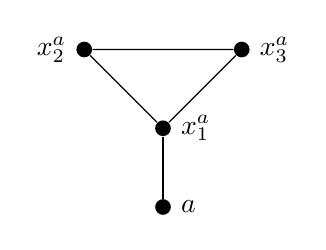
\begin{tikzpicture}
\tikzstyle{vertex}=[circle,fill=black,minimum size=1pt,inner sep=2pt]
\node[vertex,label=left:$x_2^a$] (2) at (0,0) {};
\node[vertex,label=right:$x^a_3$] (3) at (2,0) {};
\node[vertex,label=right:$x^a_1$] (1) at (1,-1) {};
\node[vertex,label=right:$a$] (a) at (1,-2) {};
\draw (2) -- (3) -- (1) -- (2);
\draw (a) -- (1);
\end{tikzpicture}
\end{center}

If \(a<b\), then \(G_A\) will have vertices \(y_1^{a,b},y_2^{a,b},y_3^{a,b}\) and
contain the subgraph

\begin{center}
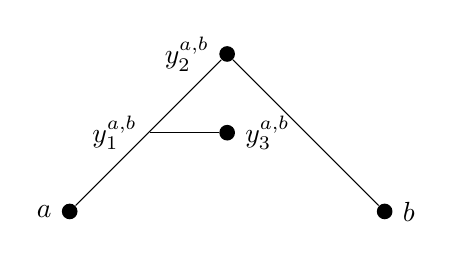
\begin{tikzpicture}
\tikzstyle{vertex}=[circle,fill=black,minimum size=1pt,inner sep=2pt]
\tikzstyle{empty}=[circle,fill=black,minimum size=1pt,inner sep=0]
\node[vertex,label=left:$y_2^{a,b}$] (2) at (2,2) {};
\node[label=left:$y_1^{a,b}$,inner sep=0] (1) at (1,1) {};
\node[vertex,label=right:$y_3^{a,b}$] (3) at (2,1) {};
\node[vertex,label=left:$a$] (a) at (0,0) {};
\node[vertex,label=right:$b$] (b) at (4,0) {};
\draw (a) -- (2);
\draw (1) -- (3);
\draw (2) -- (b);
\end{tikzpicture}
\end{center}


Let \(V_A=A\cup\{x_1^a,x_2^a,x_3^a:a\in
   A\}\cup\{y_1^{a,b},y_2^{a,b},y_3^{a,b}:a,b\in A\text{ and }a<b\}\), and let
\(R_A\) be the smallest symmetric relation containing all edges drawn above.

For example, if \(A\) is the three-element linear order \(a<b<c\), then \(G_A\) is
the graph

\begin{center}
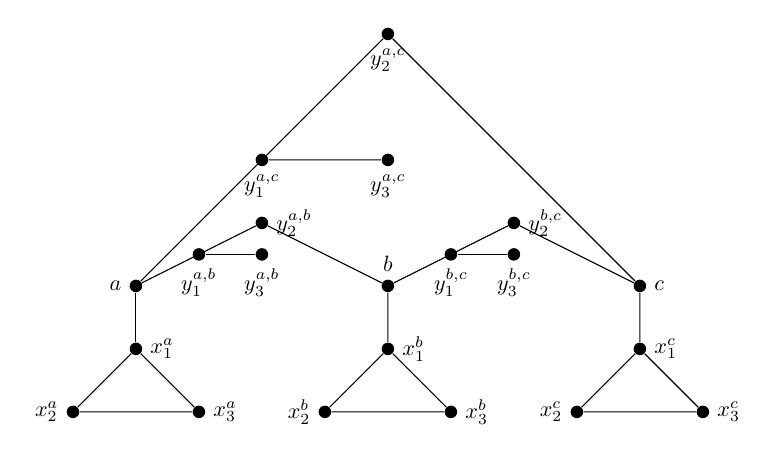
\begin{tikzpicture}[scale=0.8,transform shape]
\tikzstyle{vertex}=[circle,fill=black,minimum size=1pt,inner sep=2pt]
\tikzstyle{empty}=[circle,fill=black,minimum size=1pt,inner sep=0]
\node[vertex,label=left:$x_2^a$] (a2) at (0,0) {};
\node[vertex,label=left:$x_2^b$] (b2) at (4,0) {};
\node[vertex,label=left:$x_2^c$] (c2) at (8,0) {};
\node[vertex,label=right:$x_1^c$] (c1) at (9,1) {};
\node[vertex,label=right:$x_1^b$] (b1) at (5,1) {};
\node[vertex,label=right:$x_1^a$] (a1) at (1,1) {};
\node[vertex,label=right:$x_3^a$] (a3) at (2,0) {};
\node[vertex,label=right:$x_3^b$] (b3) at (6,0) {};
\node[vertex,label=right:$x_3^c$] (c3) at (10,0) {};
\node[vertex,label=left:$a$] (a) at (1,2) {};
\node[vertex,label=above:$b$] (b) at (5,2) {};
\node[vertex,label=right:$c$] (c) at (9,2) {};
\node[vertex,label=below:$y_1^{a,b}$] (ab1) at (2,2.5) {};
\node[vertex,label=below:$y_1^{b,c}$] (bc1) at (6,2.5) {};
\node[vertex,label=below:$y_3^{a,b}$] (ab3) at (3,2.5) {};
\node[vertex,label=right:$y_2^{a,b}$] (ab2) at (3,3) {};
\node[vertex,label=below:$y_3^{b,c}$] (bc3) at (7,2.5) {};
\node[vertex,label=right:$y_2^{b,c}$] (bc2) at (7,3) {};
\node[vertex,label=below:$y_3^{a,c}$] (ac3) at (5,4) {};
\node[vertex,label=below:$y_2^{a,c}$] (ac2) at (5,6) {};
\node[vertex,label=below:$y_1^{a,c}$] (ac1) at (3,4) {};
\draw (a2) -- (a1) -- (a3) -- (a2);
\draw (a1) -- (a);
\draw (b2) -- (b1) -- (b3) -- (b2);
\draw (b1) -- (b);
\draw (c2) -- (c1) -- (c3) -- (c2);
\draw (c1) -- (c);
\draw (a) -- (ac2);
\draw (ac2) -- (c);
\draw (a) -- (ab2);
\draw (ab1) -- (ab3);
\draw (ac1) -- (ac3);
\draw (bc1) -- (bc3);
\draw (b) -- (bc2);
\draw (b) -- (ab2);
\draw (c) -- (bc2);
\end{tikzpicture}
\end{center}

Let \(\call=\{R\}\) where \(R\) is a binary relation. Let \(\phi(x,u,v,w)\) be the
formula asserting that \(x,u,v,w\) are distinct, there are edges
\((x,u),(u,v),(v,w),(u,w)\) and these are the only edges involving \(u,v,w\).
\(G_A\models\phi(a,x_1^a,x_2^a,x_3^a)\) for all \(a\in A\).

\(\psi(x,y,u,v,w)\) asserts that \(x,y,u,v,w\) are distinct. \((x,u),(u,v),(u,w),(v,y)\)

Define \(\theta_i(z)\) as follows:
\begin{align*}
&\theta_0(z):=\exists u\exists v\exists w\;\phi(z,u,v,w)\\
&\theta_1(z):=\exists x\exists v\exists w\;\phi(x,z,v,w)\\
&\theta_2(z):=\exists u\exists u\exists w\;\phi(x,u,z,w)\\
&\theta_3(z):=\exists x\exists y\exists v\exists w\;\psi(x,y,z,v,w)\\
&\theta_4(z):=\exists x\exists y\exists u\exists w\;\psi(x,y,u,z,w)\\
&\theta_5(z):=\exists x\exists y\exists u\exists v\;\psi(x,y,u,v,z)\\
\end{align*}
If \(a,b\in A\) and \(a<b\), then
\begin{equation*}
G_A\models\theta_0(a)\wedge\theta_1(x^a_1)\wedge\theta_2(x^a_2)\wedge
\theta_2(x^a_3)
\end{equation*}
and 
\begin{equation*}
G_A\models\theta_3(y_1^{a,b})\wedge\theta_4(y_2^{a,b})\wedge\theta_5(
y_3^{a,b})
\end{equation*}
\begin{lemma}[]
If \((A,<)\) is a linear order, then for all vertices \(x\) in \(G\), there is a
unique \(i\le 5\) s.t. \(G_A\models\theta_i(x)\)
\end{lemma}

Let \(T\) be the \(\call\)-theory with the following axioms
\begin{enumerate}
\item \(R\) is symmetric and irreflexive
\item for all \(x\), exactly one \(\theta_i\) holds
\item if \(\theta_0(x)\) and \(\theta_0(y)\) then \(\neg R(x,y)\)
\item if \(\exists u\exists v\exists w\;\psi(x,y,u,v,w)\\\) then
\(\forall u_1\forall v_1\forall w_1\neg\psi(y,x,u_1,v_1,w_1)\)
\item if \(\exists u\exists v\exists w\;\psi(x,y,u,v,w)\) and 
\(\exists u\exists v\exists w\;\psi(y,z,u,v,w)\) then\par
\(\exists u\exists v\exists w\;\psi(x,z,u,v,w)\)
\item if \(\theta_0(x)\) and \(\theta_0(y)\), then either \(x=y\) or 
\(\exists u\exists v\exists w\;\psi(x,y,u,v,w)\) or
\(\exists u\exists v\exists w\;\psi(y,x,u,v,w)\)
\item if \(\phi(x,u,v,w)\wedge\phi(x,u',v',w')\), then
\(u=u',v=v',w=w'\)
\item if \(\psi(x,y,u,v,w)\wedge\psi(x,y,u',v',w')\), then
\(u'=u,v=v',w=w'\)
\end{enumerate}


If \((A,<)\) is a linear order, then \(G_A\models T\)

Suppose \(G\models T\). Let \(X_G=\{x\in G:G\models\theta_0(x)\}\)

\begin{lemma}[]
If \((A,<)\) is a linear order, then \((X_{G_A},<_{G_A})\cong(A,<)\). Moreover,
\(G_{X_G}\cong G\) for all \(G\models T\)
\end{lemma}

\begin{definition}[]
An \(\call_0\)-structure \(\caln\) is \textbf{interpretable} in an
\(\call\)-structure \(M\) if there is a definable \(X\subseteq M^n\), a definable
equivalence relation \(E\) on \(X\), and for each symbol of \(\call_0\) we can find
definable \(E\)-invariant sets on X s.t. \(X/E\) with the induced structure is
isomorphic to \(\caln\)
\end{definition}
\subsection{Answers to Exercises}
\label{sec:org323be85}
\begin{exercise}
\begin{enumerate}
\item transform \(\psi\) to CNF
\item prenex normal form
\end{enumerate}
\end{exercise}
\begin{exercise}
\begin{enumerate}
\item 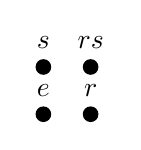
\begin{tikzpicture}[scale=0.6]
\tikzstyle{vertex}=[circle,fill=black,minimum size=1pt,inner sep=2pt]
\node[vertex,label=above:$s$] (1) at (0,1) {};
\node[vertex,label=above:$e$] (0) at (0,0) {};
\node[vertex,label=above:$r$] (2) at (1,0) {};
\node[vertex,label=above:$rs$] (3) at (1,1) {};
\end{tikzpicture}
\item enumerate \(\calm\)'s functions, relations and constants
\end{enumerate}
\end{exercise}
\begin{exercise}
\footnote{\href{https://math.stackexchange.com/questions/1170953/let-alpha-be-any-cardinal-there-are-at-most-2-alpha-cup-mathscrl}{stackexchange}}
Note that every \(\call\)-structure \(\calm\) of size \(\kappa\) is isomorphic to an
\(\call\)-structure with domain \(\kappa\). For each relation symbols, we have \(2^\kappa\)
options. If the language has size \(\lambda\), this is at most 
\((2^\kappa)^\lambda=2^{\kappa\cdot\lambda}=2^{\max(\lambda,\kappa)}\)
\end{exercise}

\begin{exercise}
\begin{align*}
T\models\phi&\Leftrightarrow\forall \calm\;\calm\models T\to\calm\models\phi\\
&\Leftrightarrow\forall \calm\;\calm\models T'\to\calm\models\phi\\
&\Leftrightarrow T'\models\phi
\end{align*}
\end{exercise}
\begin{exercise}
Follow the definition
\end{exercise}

\begin{exercise}
Since there is no model \(\calm\) s.t. \(\calm\models T\). It's true that 
\(T\models \phi\)
\end{exercise}

\begin{exercise}
\begin{enumerate}
\item Suppose \(\calm\models\phi\), then \(E^\calm\) is an equivalent relation and
each equivalence class's cardinality is 2
\item follows from number theory
\item \cite{DBLP:journals/bsl/DurandJMM12}
\end{enumerate}
\end{exercise}

\begin{exercise}
TBD
\end{exercise}

\begin{exercise}
\(G(f)=\{(\bar{x},\bar{y})\in M^{n+m}\mid\phi(\bar{x},\bar{y})\}\) and 
\(G(g)=\{(\bar{y},\bar{z})\in M^{m+l}\mid\psi(\bar{y},\bar{z})\}\). Hence
\(G(g\circ f)=\{(\bar{x},\bar{z})\in M^{n+l}\mid \phi(\bar{x},\bar{y})
   \wedge \psi(\bar{y},\bar{z})\}\)
\end{exercise}

\begin{exercise}
\(\phi(\bar{a},b)\) really defines a function and since 
\(\phi(\bar{a},y)\to y=b\)
\end{exercise}

\section{Basic Techniques}
\label{sec:org2a9d869}
\subsection{The Compactness Theorem}
\label{sec:org8605656}

\index{recursive}
A language \(\call\) is \textbf{recursive} if there is an algorithm that decides
whether a sequence of symbols is an \(\call\)-formula. An \(\call\)-theory
\(T\) is \textbf{recursive} if there is an algorithm that when given an
\(\call\)-sentence \(\phi\) as input, decides whether \(\phi\in T\)

\begin{proposition}[]
\label{prop2.1.1}
If \(\call\) is a recursive language and \(T\) is a recursive \(\call\)-theory,
then \(\{\phi:T\vdash\phi\}\) is recursively enumerable; that is, there is an
algorithm that when given \(\phi\) as input will halt accepting if \(T\vdash\phi\)
and not halt if \(T\not\vdash\phi\)
\end{proposition}
\begin{proof}
There is \(\sigma_0,\sigma_1,\dots\) a computable listing of all finite
sequence of \(\call\)-formulas. At stage \(i\), we check to see whether
\(\sigma_i\) is a proof of \(\psi\) from \(T\). If it is, then halt.
\end{proof}

\begin{theorem}[Gödel's Completeness Theorem]
Let \(T\) be an \(\call\)-theory and \(\phi\) an \(\call\)-sentence, then
\(T\models\phi\) if and only if \(T\vdash \phi\)
\end{theorem}

We say that an \(\call\)-theory \(T\) is \textbf{inconsistent} if
\(T\vdash(\phi\wedge\neg\phi)\) for some sentence \(\phi\).

\begin{corollary}[]
\(T\) is consistent if and only if \(T\) is satisfiable
\end{corollary}

\begin{proof}
Supose that \(T\) is not satisfiable, then every model of \(T\) is a model of
\(\phi\wedge\neg\phi\). Thus by the Completeness theorem
\(T\vdash(\phi\wedge\neg\phi)\) 
\end{proof}


\begin{theorem}[Compactness Theorem]
\(T\) is satisfiable if and only if every finite subset of \(T\) is satisfiable
\end{theorem}

\begin{proof}
If \(T\) is not satisfiable, then \(T\) is inconsistent. Let \(\sigma\) be a proof of
a contradiction from  \(T\). Because \(\sigma\) is finite, only finitely many
assumptions from \(T\) are used in the proof. Thus there is a finite
\(T_0\subseteq T\) s.t. \(\sigma\) is a proof of a contradiction from \(T_0\)
\end{proof}

\subsubsection{Henkin Constructions}
\label{sec:org2fd7b5d}
A theory \(T\) is \textbf{finitely satisfiable} if every finite subset of \(T\) is
satisfiable. We will show that every finitely satisfiable theory \(T\) is
satisfiable.

\begin{definition}[]
We say that an \(\call\)-theory \(T\) has the \textbf{witness property} if whenever
\(\phi(v)\) is an \(\call\)-formula with one free variable \(v\), then there is
a constant symbol \(c\in\call\) s.t. \(T\vdash(\exists v\phi(v))\to\phi(c)\)

An \(\call\)-theory \(T\) is \textbf{maximal} if for all \(\phi\) either \(\phi\in T\) or
\(\neg\phi\in T\)
\end{definition}

\begin{lemma}[]
Suppose \(T\) is a maximal and finitely satisfiable \(\call\)-theory. If
\(\Delta\subseteq T\) is finite and \(\Delta\models\psi\), then \(\psi\in T\)
\end{lemma}

\begin{proof}
If \(\psi\not\in T\), then \(\neg\psi\in T\) but \(\Delta\cup\{\psi\}\) is
unsatisfiable 
\end{proof}

\begin{lemma}[]
Suppose that \(T\) is a maximal and finitely satisfiable \(\call\)-theory with
the witness property. Then \(T\) has a model. In fact, if \(\kappa\) is a cardinal
and \(\call\) has at most \(\kappa\) constant symbols, then there is
\(\calm\models T\) with \(\abs{\calm}\le\kappa\)
\end{lemma}

\begin{proof}
Let \(\calc\) be the set of constant symbols of \(\call\). For \(c,d\in\calc\),
we say \(c\sim d\) if \(T\models c=d\)

\textbf{Claim 1} \(\sim\) is an equivalence relation. 

The universe of our model will be \(M=\calc/\sim\). Clearly
\(\abs{M}\le\kappa\). We let \(c^*\) denote the equivalence class of \(c\) and
interprete \(c\) as its equivalence class, that is, \(c^\calm=c^*\)

Suppose that \(R\) is an \(n\)-ary relation symbol of \(\call\)

\textbf{Claim 2} Suppose that \(c_1,\dots,c_n,d_1,\dots,d_n\in\calc\) and \(c_i\sim d_i\)
for \(i=1,\dots,n\), then \(R(\bar{c})\) if and only if \(R(\bar{d})\)
\begin{equation*}
R^\calm=\{(c_1^*,\dots,c_n^*):R(c_1,\dots,c_n)\in T\}
\end{equation*}
Suppose that \(f\) is an \(n\)-ary function symbol of \(\call\) and
\(c_1,\dots,c_n\in\calc\). Because  \(\underline{\emptyset\models\exists
    vf(c_1,\dots,c_n)=v}\), and \(T\) has the witness property, then there is
\(c_{n+1}\in\calc\) s.t. \(f(c_1,\dots,c_n)=c_{n+1}\in T\). As above, if
\(d_i\sim c_i\) for \(i=1,\dots,n+1\), then \(f(d_1,\dots,d_n)=d_{n+1}\in T\).
Thus we get a well-defined function \(f^\calm:M^n\to M\) by
\begin{equation*}
f^\calm(c_1^*,\dots,c_n^*)=d^*\text{ if and only if }f(c_1,\dots,c_n)=d\in T
\end{equation*}

\textbf{Claim 3} Suppose that \(t\) is a term using free variables from
\(v_1,\dots,v_n\). If \(c_1,\dots,c_n,d\in\calc\), then \(t(c_1,\dots,c_n)=d\in
    T\) if and only if \(t^\calm(c_1^*,\dots,c_n^*)=d^*\)

(\(\Leftarrow\)) Suppose \(t^\calm(c_1^*,\dots,c_n^*)=d^*\). By the witness
property, there is a \(e\in\calc\) s.t. \(t(c_1,\dots,c_n)=e\in T\). Using the
\((\Rightarrow)\) direction of the proof, \(t^\calm(c_1^*,\dots,c_n^*)=e^*\).
Thus \(e^*=d^*\) and \(e=d\in T\)


\textbf{Claim 4} For all \(\call\)-formulas \(\phi(v_1,\dots,v_n)\) and
 \(c_1,\dots,c_n\in\calc\), \(\calm\models\phi(\bar{c}^*)\) if and only if
 \(\phi(\bar{c})\in T\)
\end{proof}

\begin{lemma}[]
Let \(T\) be a finitely satisfiable \(\call\)-theory. There is a language
\(\call^*\supseteq\call\) and \(T^*\supseteq T\) a finitely satisfiable
\(\call^*\)-theory s.t. any \(\call^*\)-theory extending \(T^*\) has the
witness property. We can choose \(\call^*\) s.t.
\(\abs{\call^*}=\abs{\call}+\aleph_0\) 
\end{lemma}

\begin{proof}
We first show that there is a language \(\call_1\supseteq\call\) and a
finitely satisfiable \(\call_1\)-theory \(\call_1\supseteq T\) s.t. for any
\(\call\)-formula \(\phi(v)\) there is an \(\call_1\)-constant symbol \(c\) s.t.
\(T_1\models(\exists v\phi(v))\to\phi(c)\). For each \(\call\)-formula
\(\phi(v)\), let \(c_\phi\) be a new constant symbol and let
\(\call_1=\call\cup\{c_\phi:\phi(v)\text{ an }\call\text{-formula}\}\). For
each \(\call\)-formula \(\phi(v)\), let \(\Theta_\phi\) be the
\(\call_1\)-sentence
\((\exists v\phi(v))\to\phi(c_\phi)\). Let
\(T_1=T\cup\{\Theta_\phi:\phi(v)\text{ an }\call\text{-formula}\}\)

\textbf{Claim} \(T_1\) is finitely satisfiable

Suppose that \(\Delta\) is a finite subset of \(T_1\). Then
\(\Delta=\Delta_0\cup\{\Theta_{\phi_1},\dots, \Theta_{\phi_n}\}\) where
\(\Delta_0\) is a finite subset of \(T\) and there is \(\calm\models\Delta_0\). We
will make \(\calm\) into an
\(\call\cup\{c_{\phi_1},\dots,c_{\phi_n}\}\)-structure \(\calm'\). If
\(\calm\models\exists v\phi(v)\), choose \(a_i\) some element of \(M\) s.t.
\(\calm\models\phi(a_i)\) and let \(c_{\phi_i}^{\calm'}=a_i\). Otherwise, let
\(c_{\phi_i}^{\calm'}\) be any element of \(\calm\). Clearly
\(\calm'\models\Theta_{\phi_i}\) for \(i\le n\). Thus \(T_1\) is finitely
satisfiable.

We now iterate the construction above to build a sequence of languages
\(\call\subseteq\call_1\subseteq\call_2\subseteq\dots\) and a sequence of
finitely satisfiable \(\call_i\)-theories \(T\subseteq T_1\subseteq
    T_2\subseteq\dots\) s.t. if \(\phi(v)\) is an \(\call_i\)-formula then there is
a constant symbol \(c\in\call_{i+1}\) s.t. \(T_{i+1}\models(\exists
    v\phi(v))\to\phi(c)\)

Let \(\call^*=\bigcup\call_i\) and \(T^*=\bigcup T_i\). And by induction,
\(\abs{\call^*}=\abs{\call}+\aleph_0\) 
\end{proof}

\begin{lemma}[]
Suppose that \(T\) is a finitely satisfiable \(\call\)-theory and \(\phi\) is an
\(\call\)-sentence, then either \(T\cup\{\phi\}\) or \(T\cup\{\neg\phi\}\) is
finitely satisfiable
\end{lemma}

\begin{corollary}[]
If \(T\) is a finitely satisfiable \(\call\)-theory, then there is a maximal
finitely satisfiable \(\call\)-theory \(T'\supseteq T\)
\end{corollary}
\begin{proof}
Let \(I\) be the set of all finitely satisfiable \(\call\)-theory containing
\(T\). We partially order \(I\) by inclusion. If \(C\subseteq I\) is a chain, let
\(T_C=\bigcup\{\Sigma:\Sigma\in C\}\). If \(\Delta\) is a finite subset of
\(T_C\), then there is a \(\Sigma\in C\) s.t. \(\Delta\subseteq\Sigma\), so \(T_C\)
is finitely satisfiable and \(T_C\supseteq\Sigma\) for all \(\Sigma\in C\). Thus
every chain in \(I\) has an upper bound, and we can apply Zorn's lemma to find
a \(T'\in I\) maximal w.r.t. the partial order.
\end{proof}


\begin{theorem}[stengthening of Compactness Theorem]
\label{thm2.1.11}
If \(T\) is a finitely satisfiable \(\call\)-theory and \(\kappa\) is an infinite
cardinal with \(\kappa\ge\abs{\call}\), then there is a model of \(T\) of
cardinality at most \(\kappa\)
\end{theorem}

\begin{proposition}[]
Let \(\call=\{\cdot,+,<,0,1\}\) and let \(\Th(\N)\) be the full \(\call\)-theory
of the natural numbers. There is \(\calm\models\Th(\N)\) and \(a\in M\) s.t. \(a\)
is larget than every natural number
\end{proposition}

\begin{proof}
Let \(\call^*=\call\cup\{c\}\) where \(c\) is a new constant symbol and let
\begin{equation*}
T=\Th(\N)]\cup\{\underbrace{1+1+\dots+1}_{n\text{-times}}<c:\text{for }n=1,2,\dots\} 
\end{equation*}
If \(\Delta\) is a finite subset of \(T\) we can make \(\N\) a model of \(\Delta\) by
interpreting \(c\) as a suitably large natural number. Thus \(T\) is finitely
satisfiable and there is \(\calm\models T\).
\end{proof}
\begin{lemma}[]
If \(T\models\phi\), then \(\Delta\models T\) for some finite \(\Delta\subseteq T\)
\end{lemma}
\begin{proof}
Suppose not. Let \(\Delta\subseteq T\) be finite. Because
\(\Delta\not\models\phi\), \(\Delta\cup\{\neg\phi\}\) is satisfiable. Thus
\(T\cup\{\neg\phi\}\) is finitely satisfiable and by the compactness theorem,
\(T\not\models\phi\) 
\end{proof}



\subsection{Complete Theories}
\label{sec:org1076959}
\begin{definition}[]
An \(\call\)-theory \(T\) is called \textbf{complete} if for any \(\call\)-sentence \(\phi\)
either \(T\models\phi\) or \(T\models\neg\phi\)
\end{definition}

For \(\calm\) an \(\call\)-structure, then the full theory
\begin{equation*}
\Th(\calm)=\{\phi:\phi\text{ is an }\call\text{-sentence and }
\calm\models\phi\}
\end{equation*}
is a complete theory.

\begin{proposition}[]
\label{prop2.2.2}
Let \(T\) be an \(\call\)-theory with infinite models. If \(\kappa\) is an infinite
cardinal and \(\kappa\ge\abs{\call}\), then there is a model of \(T\) of
cardinality \(\kappa\)
\end{proposition}

\begin{proof}
Let \(\call^*=\call\cup\{c_\alpha:\alpha<\kappa\}\), where each \(c_\alpha\) is
new constant symbol, and let \(T^*\) be the \(\call^*\)-theory
\(T\cup\{c_\alpha\neq c_\beta:\alpha,\beta<\kappa,\alpha\neq\beta\}\). Clearly
if \(\calm\models T^*\), then \(\calm\) is a model of \(T\) of cardinality at least
\(\kappa\).
Thus by Theorem \ref{thm2.1.11}, it suffices to show that \(T^*\) is finitely
satisfiable. But if \(\Delta\subseteq T^*\) is finite, then \(\Delta\subseteq
   T\cup\{c_\alpha\neq c_\beta:\alpha\neq\beta,\alpha,\beta\in I\}\), where \(I\)
is a finite subset of \(\kappa\). Let \(\calm\) be an infinite model of \(T\). We can
interpret the symbols \(\{c_\alpha:\alpha\in I\}\) as \(\abs{I}\) distinct
elements of \(M\). Because \(\calm\models\Delta\), \(T^*\) is finitely satisfiable.
\end{proof}

\begin{definition}[]
Let \(\kappa\) be an infinite cardinal and let \(T\) be a theory with models of
size \(\kappa\). We say that \(T\) is \textbf{\(\kappa\)-categorical} if any two models of
\(T\) of cardinality \(\kappa\) are isomorphic.
\end{definition}

Let \(\call=\{+,0\}\) be the language of additive groups and let \(T\) be the
\(\call\)-theory of torsion-free divisible Abelian groups. The axioms of \(T\)
are the axioms for Abelian groups together with the axioms
\begin{gather*}
\forall x(x\neq 0\to\underbrace{x+\dots+x}_{n\text{-times}}\neq 0)\\
\forall y\exists x\underbrace{x+\dots+x}_{n\text{-times}}=y
\end{gather*}
for \(n=1,2,\dots\)


\begin{proposition}[]
The theory of torsion-free divisible Abelian groups is \(\kappa\)-categorical for
all \(\kappa>\aleph_0\)
\end{proposition}

\begin{proof}
We first argue that models of \(T\) are essentially vector spaces over the
field of rational numbers \(\Q\). If \(V\) is any vector space over \(\Q\), then
the underlying additive group \(V\) is a model of \(T\). 
Check \href{https://math.stackexchange.com/questions/1550900/necessary-and-sufficient-conditions-for-an-abelian-group-to-be-a-vector-space-ov/1550954}{StackExchange}.
On the other hand, if
\(G\models T\), \(g\in G\) and \(n\in\N\) with \(g>0\), we can find 
\(h\in G\) s.t. \(nh=g\). If \(nk=g\), then \(n(h-k)=0\). Because \(G\) is
torsion-free there is a unique \(h\in G\) s.t. \(nh=g\). We call this element 
\(g/n\). We can view \(G\) as a \(\Q\)-vector space under the action
\(\frac{m}{n}g=m(g/n)\)

Two \(\Q\)-vector spaces are isomorphic if and only if they have the same
dimension. Thus the model of \(T\) are determined up to isomorphism by their
dimension. If \(G\) has dimension \(\lambda\), then \(\abs{G}=\lambda+\aleph_0\). If \(\kappa\)
is uncountable and \(G\) has cardinality \(\kappa\), then \(G\) has dimension \(\kappa\). Thus for
\(\kappa>\aleph_0\) any two models of \(T\) of cardinality \(\kappa\) are isomorphic
\end{proof}

\begin{proposition}[]
\(\ACF_p\) is \(\kappa\)-categorical for all uncountable cardinals \(\kappa\)
\end{proposition}

\begin{proof}
   
\end{proof}

\begin{theorem}[Vaught's Test]
Let \(T\) be a satisfiable theory with no finite models that is
\(\kappa\)-categorical for some infinite cardinal \(\kappa\ge\abs{\call}\). Then
\(T\) is complete
\end{theorem}

\begin{proof}
Suppose \(T\) is not complete. Then there is a sentence \(\phi\) s.t. 
\(T\not\models\phi\) and \(T\not\models\neg\phi\). Because
\(T\not\models\psi\) if and only if \(T\cup\{\neg\psi\}\) is satisfiable, the
theories \(T_0=T\cup\{\phi\}\) and \(T_1=T\cup\{\neg\phi\}\) are satisfiable.
Because \(T\) has no finite models, both \(T_0\) and \(T_1\) have infinite
models. By Proposition \ref{prop2.2.2} we can find \(\calm_0\) and
\(\calm_1\) of cardinality \(\kappa\) with \(\calm_i\models T_i\). Because \(\calm_0\)
and \(\calm_1\) disagree about \(\phi\), they are not elementarily equivalent, and
hence by Theorem \ref{thm1.1.10}, nonisomorphic. 
\end{proof}

\begin{definition}[]
We say that an \(\call\)-theory \(T\) is \textbf{decidable} if there is an algorithm
that when given an \(\call\)-sentence \(\phi\) as input decides whether \(T\models\phi\)
\end{definition}

\begin{lemma}[]
Let \(T\) be a recursive complete satisfiable theory in a recursive language
\(\call\). Then \(T\) is decidable
\end{lemma}

\begin{proof}
Because \(T\) is satisfiable \(A=\{\phi:T\models\phi\}\) and
\(B=\{\phi:T\models\neg\phi\}\) are disjoint. Because \(T\) is consistent 
\(A\cup B\) is the set of all \(\call\)-sentences. By the Completeness
Theorem, \(A=\{\phi:T\vdash\phi\}\) and \(B=\{\phi:T\vdash\neg\phi\}\). By
Proposition \ref{prop2.1.1} \(A\) and \(B\) are recursively enumerable. But any
recursively enumerable set with a recursively enumerable complement is
recursive. 
\end{proof}

\begin{corollary}[]
For \(p=0\) or \(p\) prime, \(ACF_p\) is decidable. In particular, \(\Th(\C)\),
the first-order theory  of the field of complex numbers, is decidable
\end{corollary}

\begin{corollary}[]
Let \(\phi\) be a sentence in the language of rings. The following are equivalent
\begin{enumerate}
\item \(\phi\) is true in the complex number
\item \(\phi\) is true in every algebraically closed field of characteristic zero
\item \(\phi\) is true in some algebraically closed field of characteristic zero
\item There are arbitrarily large primes \(p\) s.t. \(\phi\) is true in some
algebraically closed field of characteristic \(p\)
\item There is an \(m\) s.t. for all \(p>m\), \(\phi\) is true in all algebraically
closed fields of characteristic \(p\)
\end{enumerate}
\end{corollary}
\section{Reference}
\label{sec:org65db36c}
\bibliographystyle{alpha}
\bibliography{../references}
\section{Index}
\label{sec:org2171b3b}
\renewcommand{\indexname}{}
\printindex
\end{document}